% Exam Template for UMTYMP and Math Department courses
%
% Using Philip Hirschhorn's exam.cls: http://www-math.mit.edu/~psh/#ExamCls
%
% run pdflatex on a finished exam at least three times to do the grading table on front page.
%
%%%%%%%%%%%%%%%%%%%%%%%%%%%%%%%%%%%%%%%%%%%%%%%%%%%%%%%%%%%%%%%%%%%%%%%%%%%%%%%%%%%%%%%%%%%%%%

% These lines can probably stay unchanged, although you can remove the last
% two packages if you're not making pictures with tikz.
\documentclass[11pt]{exam}
\usepackage{multirow}  
\usepackage{array}
\newcolumntype{x}[1]{>{\centering\arraybackslash\hspace{0pt}}p{#1}}
\usepackage{slashbox,booktabs,amsmath}
\RequirePackage{amssymb, amsfonts, amsmath, latexsym, verbatim, xspace, setspace}
\RequirePackage{tikz, pgflibraryplotmarks}
\usepackage[]{algorithm2e}
\usepackage{subfigure}
\usepackage[]{algorithmic}
		\usepackage{graphicx}
% By default LaTeX uses large margins.  This doesn't work well on exams; problems
% end up in the "middle" of the page, reducing the amount of space for students
% to work on them.
\usepackage[margin=1in]{geometry}

\usepackage{graphicx}



% Here's where you edit the Class, Exam, Date, etc.
\newcommand{\university}{Universidad Industrial de Santander}
\newcommand{\class}{Mathematical modelling}
\newcommand{\term}{2018- II}
\newcommand{\examnum}{Workshop No. 1 - Root-finding Methods }
\newcommand{\examdate}{\today}
\newcommand{\timelimit}{30 minutos}
\newcommand{\fechaentrega}{--/--/--}
\newcommand{\proffesor}{Professor: Juan Carlos Basto Pineda}
\pointpoints{punto}{points}
\vpword{Points} 
\vsword{Grade}
\hpword{points}
 
% For an exam, single spacing is most appropriate
\singlespacing
% \onehalfspacing
% \doublespacing

% For an exam, we generally want to turn off paragraph indentation
\parindent 0ex

\begin{document} 

% These commands set up the running header on the top of the exam pages
\pagestyle{head}
\firstpageheader{}{}{}
\runningheader{\class}{\examnum}{\examdate}
\runningheadrule
\begin{center}
\begin{minipage}[t]{2.8in}
\vspace{0pt}
\textbf{\university} \\
\textbf{\proffesor} \\
\textbf{\term} \\
\end{minipage}
\hfill
\begin{minipage}[t]{3.4in}
\vspace{0pt}
\textbf{\examnum} \\
\textbf{\class}  \\
%\textbf{Tiempo l\'imite: \timelimit}  \\
\textbf{Date: \examdate} \\
%\textbf{\fechaentrega}
\end{minipage}
\end{center}
\vspace{0.2in}
\textbf{Name:} \makebox[4.0in]{Andr\'es Felipe Jerez Ariza} \textbf{Scholar ID:} \makebox[1.5 in]{2188136}\\ 


 % End of cover page

%%%%%%%%%%%%%%%%%%%%%%%%%%%%%%%%%%%%%%%%%%%%%%%%%%%%%%%%%%%%%%%%%%%%%%%%%%%%%%%%%%%%%
%
% See http://www-math.mit.edu/~psh/#ExamCls for full documentation, but the questions
% below give an idea of how to write questions [with parts] and have the points
% tracked automatically on the cover page.
%
%
%%%%%%%%%%%%%%%%%%%%%%%%%%%%%%%%%%%%%%%%%%%%%%%%%%%%%%%%%%%%%%%%%%%%%%%%%%%%%%%%%%%%%
\section{Introduction}
In mathematics and computing, a root-finding algorithm is an algorithm for finding roots of continuous functions. A root of a function $f$, from the real numbers to real numbers or from the complex numbers to the complex numbers, is a number $x$ such that $f(x) = 0$. As, generally, the roots of a function cannot be computed exactly, nor expressed in closed form, root-finding algorithms provide approximations to roots, expressed either as floating point numbers or as small isolating intervals, or disks for complex roots (an interval or disk output being equivalent to an approximate output together with an error bound).\\\\
In order to solve the root-finding problem was developed many algorithms based on bracketing methods, iterative methods and combinations of methods. 

\begin{itemize}
	\item \textbf{Bracketing methods:} determine successively smaller intervals (brackets) that contain a root, e.g., bisection method.
	\item \textbf{Iterative methods:} an iterative root-finding method generally use a specific type of iteration, consisting of defining an auxiliary function, which is applied to the last computed approximations of a root for getting a new approximation, e.g., Newton-Rhapson and secant methods.
	\item \textbf{Combinations of methods:} Brent's method is a combination of the bisection method, the secant method and inverse quadratic interpolation. At every iteration, Brent's method decides which method out of these three is likely to do best, and proceeds by doing a step according to that method. 
\end{itemize}

In this work, some root-finding algorithms were implemented such as the bisection method, the secant method, Newton method and Brent's method. Several simulations were carried out in order to evaluate each algorithm according to convergence order, number of iteration, absolute error, and tolerance using four different functions, which are given by

\begin{equation}\label{f1}
f_1(x)=x^2-2,
\end{equation}
\begin{equation}\label{f2}
f_2(x)=x^3-10x^2+5,
\end{equation}
\begin{equation}\label{f3}
f_3(x)=e^x\sin(x)+4,
\end{equation}
\begin{equation}\label{f4}
f_4(x)=\cosh(x)\cos(x)-1,
\end{equation}

In Fig. \ref{fig:function} the sketches of these functions including its roots is presented.

\begin{figure}[!h]
	\centering
	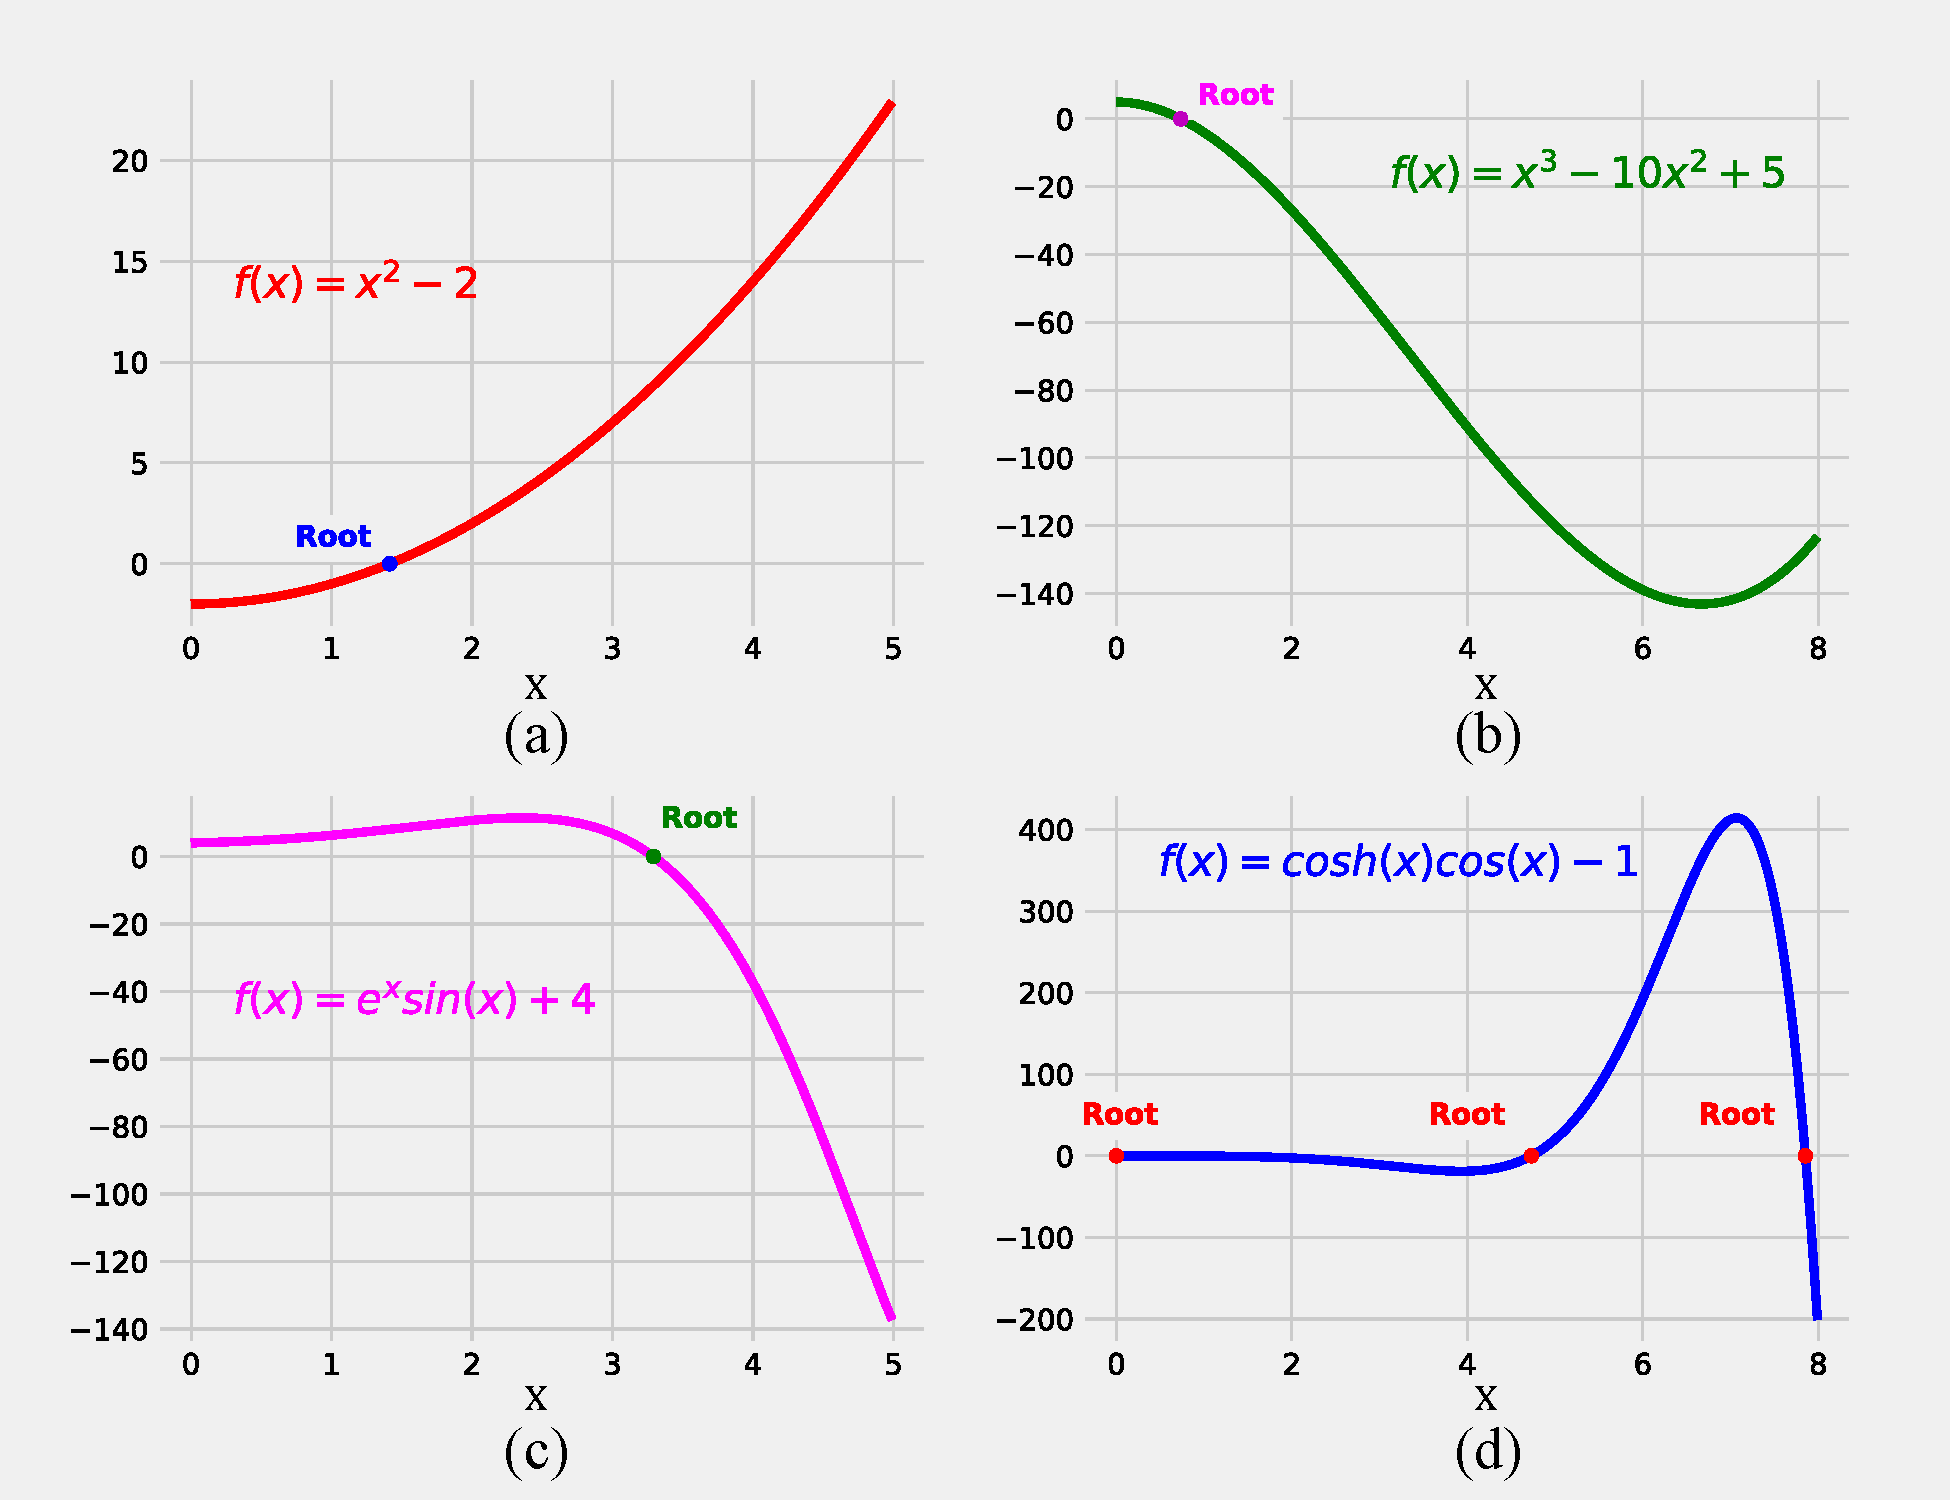
\includegraphics[width=12cm]{img/Functions.pdf}\caption{Implemented functions in order to evaluate different root-finding algorithms.}\label{fig:function}
\end{figure}

\section{Results}
In order to evaluate the performance of the bisection method, secant method, Newton method and Brent's method, several simulations were tested. Therefore, absolute error, convergence order, and tolerance were estimated to compare the performance of the implemented algorithms. These metrics are recalled as follow


\begin{itemize}
	\item Absolute error
	\begin{equation}\label{eq:absolute}
	e_k=\left | \tilde{x}_k-x \right |,
	\end{equation}
	where $\tilde{x}_k\in\mathbb{R}$ represents the approximation root in the $k$-th iteration and $x\in\mathbb{R}$ is the real root.
	\item Convergence order
	\begin{equation}\label{eq:convergence}
	\lim_{k\rightarrow \infty }\frac{\left | e_{k+1} \right |}{\left | e_k \right |^r}=C,
	\end{equation}
	where $r\in\mathbb{R}$ corresponds to convergence order and $C\in\mathbb{R}$ is a constant.
	\item Tolerance:
	\begin{equation}\label{eq:tolerance}
	\delta_k=\left | \tilde{x}_k-\tilde{x}_{k-1} \right |,
	\end{equation}
\end{itemize}

Notice that the convergence order using Eq. \ref{eq:convergence} cannot be directly evaluated. Then, Eq. \ref{eq:convergence} is reorganized using the logarithmic function as
\begin{equation}\label{eq:ratio}
e_{k+1}=Ce_k^r\rightarrow \log(e_{k+1})=\log(C)+r\log(e_k),
\end{equation}

In table \ref{tb:iterations} the number of iterations at each root-finding method is presented using a tolerance $\delta=10^{-4}$. Bisection method requires up to 15 iterations, while Brent's method just requires up to 7 iterations to find a root under this tolerance. In table \ref{tb:convergence} the convergence order at each root-finding method is shown using a tolerance $\delta=10^{-4}$. Bisection method requires up to 15 iterations, while Brent's method just requires up to 7. The mean and standard deviation (STD) of the convergence order according to each function and method was calculated. Taken the low difference between experimental and theoretical convergence order into account, the reliability of the simulation results of these methods is can be guaranteed.


\begin{table}[h!]
	\centering
	\begin{tabular}{l|l|l|l|l|}
		\cline{2-5}
		& \multicolumn{4}{c|}{\textbf{Iterations}}                                                                                        \\ \hline
		\multicolumn{1}{|c|}{\textbf{Method}} & \multicolumn{1}{c|}{$f_1$} & \multicolumn{1}{c|}{$f_2$} & \multicolumn{1}{c|}{$f_3$} & \multicolumn{1}{c|}{$f_4$} \\ \hline
		\multicolumn{1}{|l|}{Bisection}       & 15                        & 15                        & 12                                 & 14                                 \\ \hline
		\multicolumn{1}{|l|}{Secant}          & 7                         & 7                         & 4                                  & 7                                  \\ \hline
		\multicolumn{1}{|l|}{Newton}          & 8                         & 6                         & 3                                  & 5                                  \\ \hline
		\multicolumn{1}{|l|}{Brent}           & 6                         & 7                         & 4                                  & 7                                  \\ \hline
	\end{tabular}\caption{Amount of iteration at each root-finding method using $\delta=10^{-4}$.}\label{tb:iterations}
\end{table}


\begin{table}[!h]
	\centering
	\begin{tabular}{l|c|c|c|c|c|c|c|c|}
		\cline{2-9}
		& \multicolumn{8}{c|}{\textbf{Convergence order}}                                                                                   \\ \hline
		\multicolumn{1}{|c|}{\textbf{Method}} & f\_1   & f\_2   & f\_3   & f\_4   & \textbf{Mean}                 & \textbf{STD} & \textbf{Real}                 & \textbf{Error} \\ \hline
		\multicolumn{1}{|l|}{Bisection}       & 0,7413 & 0,6860 & 0,6088 & 0,8036 & {\color[HTML]{3166FF} 0,7099} & 0,0828       & {\color[HTML]{CE6301} 0,5000} & 0,2099         \\ \hline
		\multicolumn{1}{|l|}{Secant}          & 1,5987 & 1,4727 & 1,6182 & 1,6249 & {\color[HTML]{3166FF} 1,5786} & 0,0715       & {\color[HTML]{CE6301} 1,6180} & 0,0394         \\ \hline
		\multicolumn{1}{|l|}{Newton}          & 1,9304 & 1,9128 & 1,9978 & 1,9881 & {\color[HTML]{3166FF} 1,9573} & 0,0420       & {\color[HTML]{CE6301} 2,0000} & 0,0427         \\ \hline
		\multicolumn{1}{|l|}{Brent}           & 1,8647 & 1,8446 & 1,7943 & 1,8258 & {\color[HTML]{3166FF} 1,8324} & 0,0299       & {\color[HTML]{CE6301} 1,8393} & 0,0069         \\ \hline
	\end{tabular}\caption{Convergence order at each root-finding method using $\delta=10^{-4}$.}\label{tb:convergence}
\end{table}

In Fig \ref{fig:deltaVsiter} the comparison between tolerance $\delta_k$ and iteration using a maximum tolerance $\delta=10^{-4}$ is illustrated. In Fig \ref{fig:errVsiter} the comparison between absolute error $e_k$ and iteration using a maximum tolerance $\delta=10^{-4}$ is presented. On the other hand, in Fig \ref{fig:errVserr} the relationship between $e_{k+1}$ and $e_k$ using Eq. \ref{eq:ratio} to estimate the convergence order $r$ is shown. Then, the convergence order is given by the slope of the linear fitting according to each root-finding algorithm. Furthermore, in Fig \ref{fig:timeVsdelta} the time measured in seconds of the performance of the tested root-finding methods according to tolerance $\delta=\{10^{-1},10^{-2},10^{-3},10^{-4}\}$ is illustrated. Notice that the time increases when we have a low tolerance. However, the Newton method by using Eq. \ref{f1} produces a different behavior. In general, the Newton method, secant method, and Brent's method produce an almost constant time according to tolerance.

\begin{figure}[!h]
	\centering
	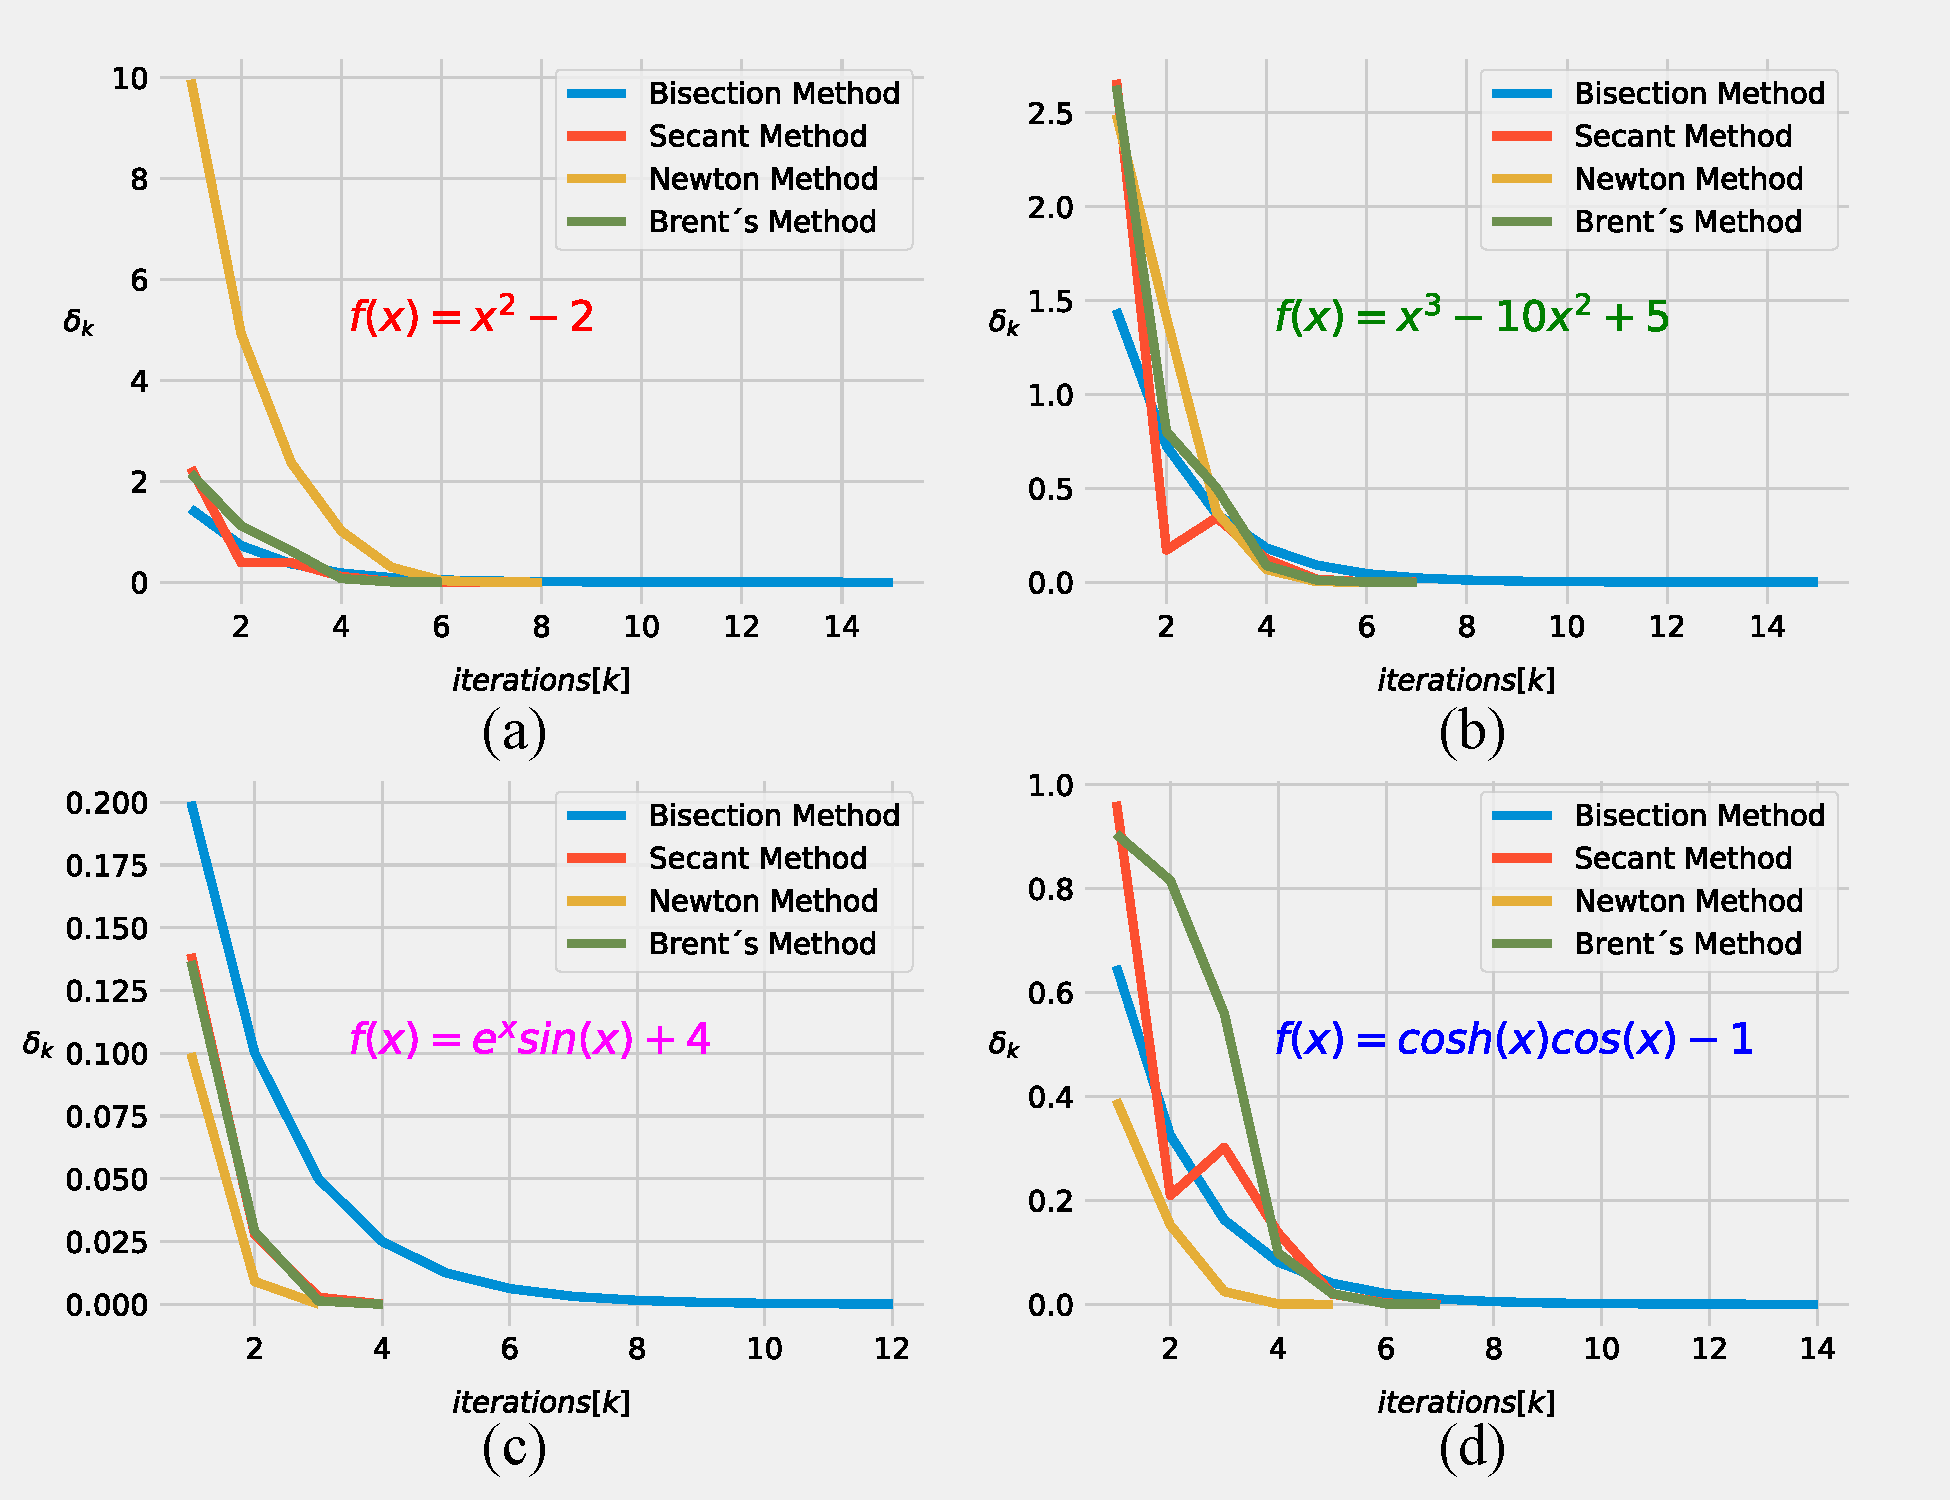
\includegraphics[width=12cm]{img/DeltaVsIter.pdf}\caption{Comparison between $\delta_k$ and iteration using different root-finding algorithms and functions. }\label{fig:deltaVsiter}
\end{figure}
\begin{figure}[!h]
	\centering
	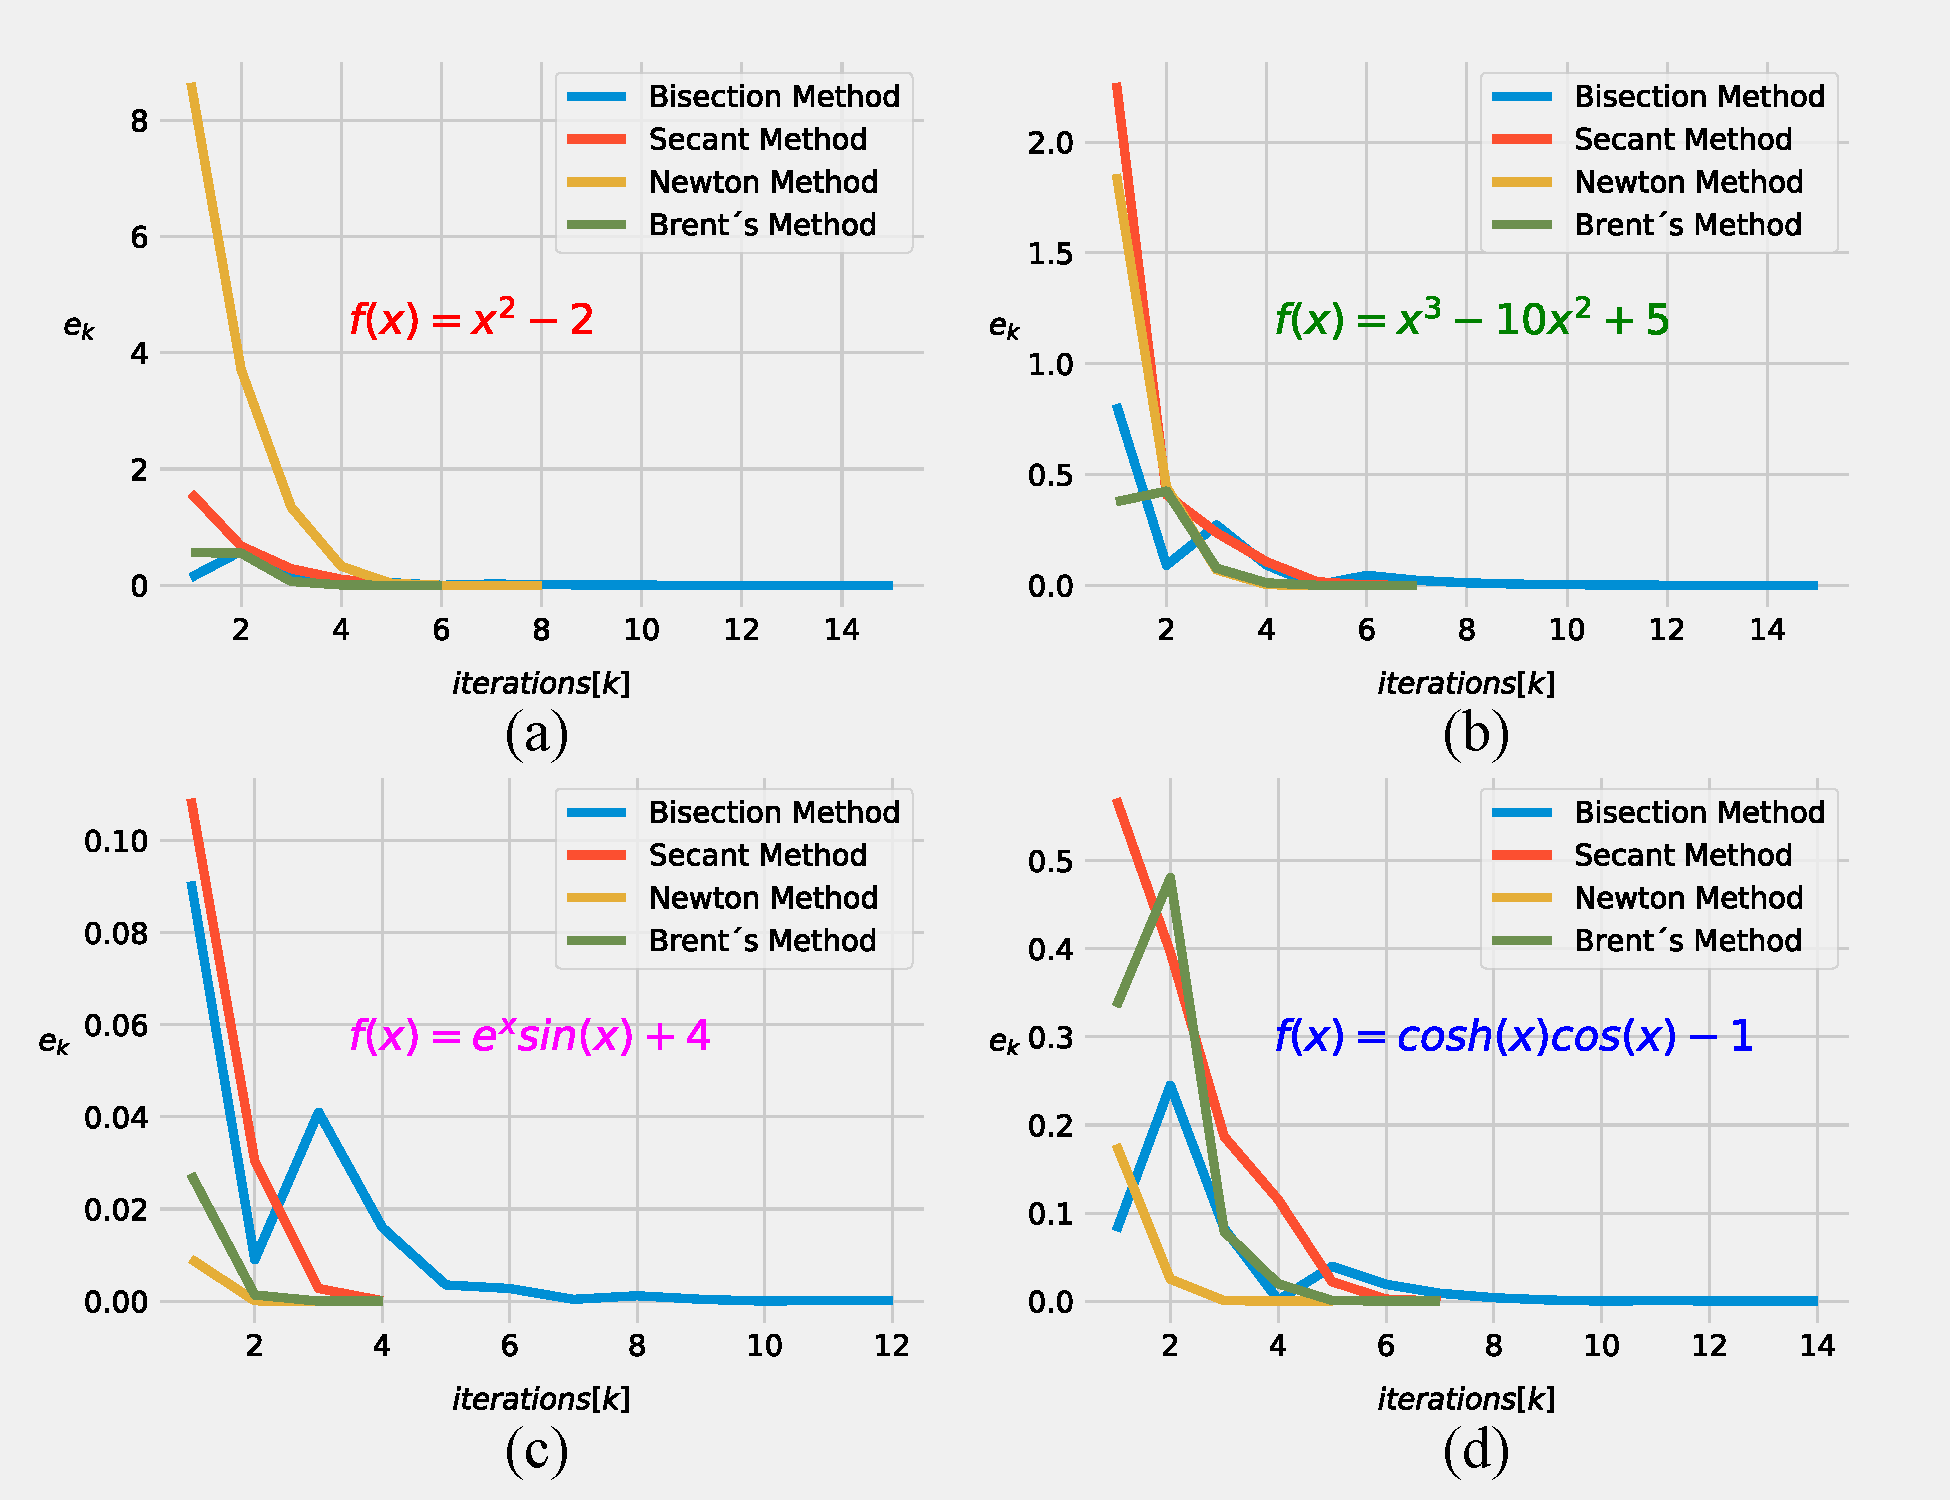
\includegraphics[width=12cm]{img/ErrorVsIter.pdf}\caption{Comparison between $e_k$ and iteration using different root-finding algorithms and functions. }\label{fig:errVsiter}
\end{figure}

\begin{figure}[!h]
	\centering
	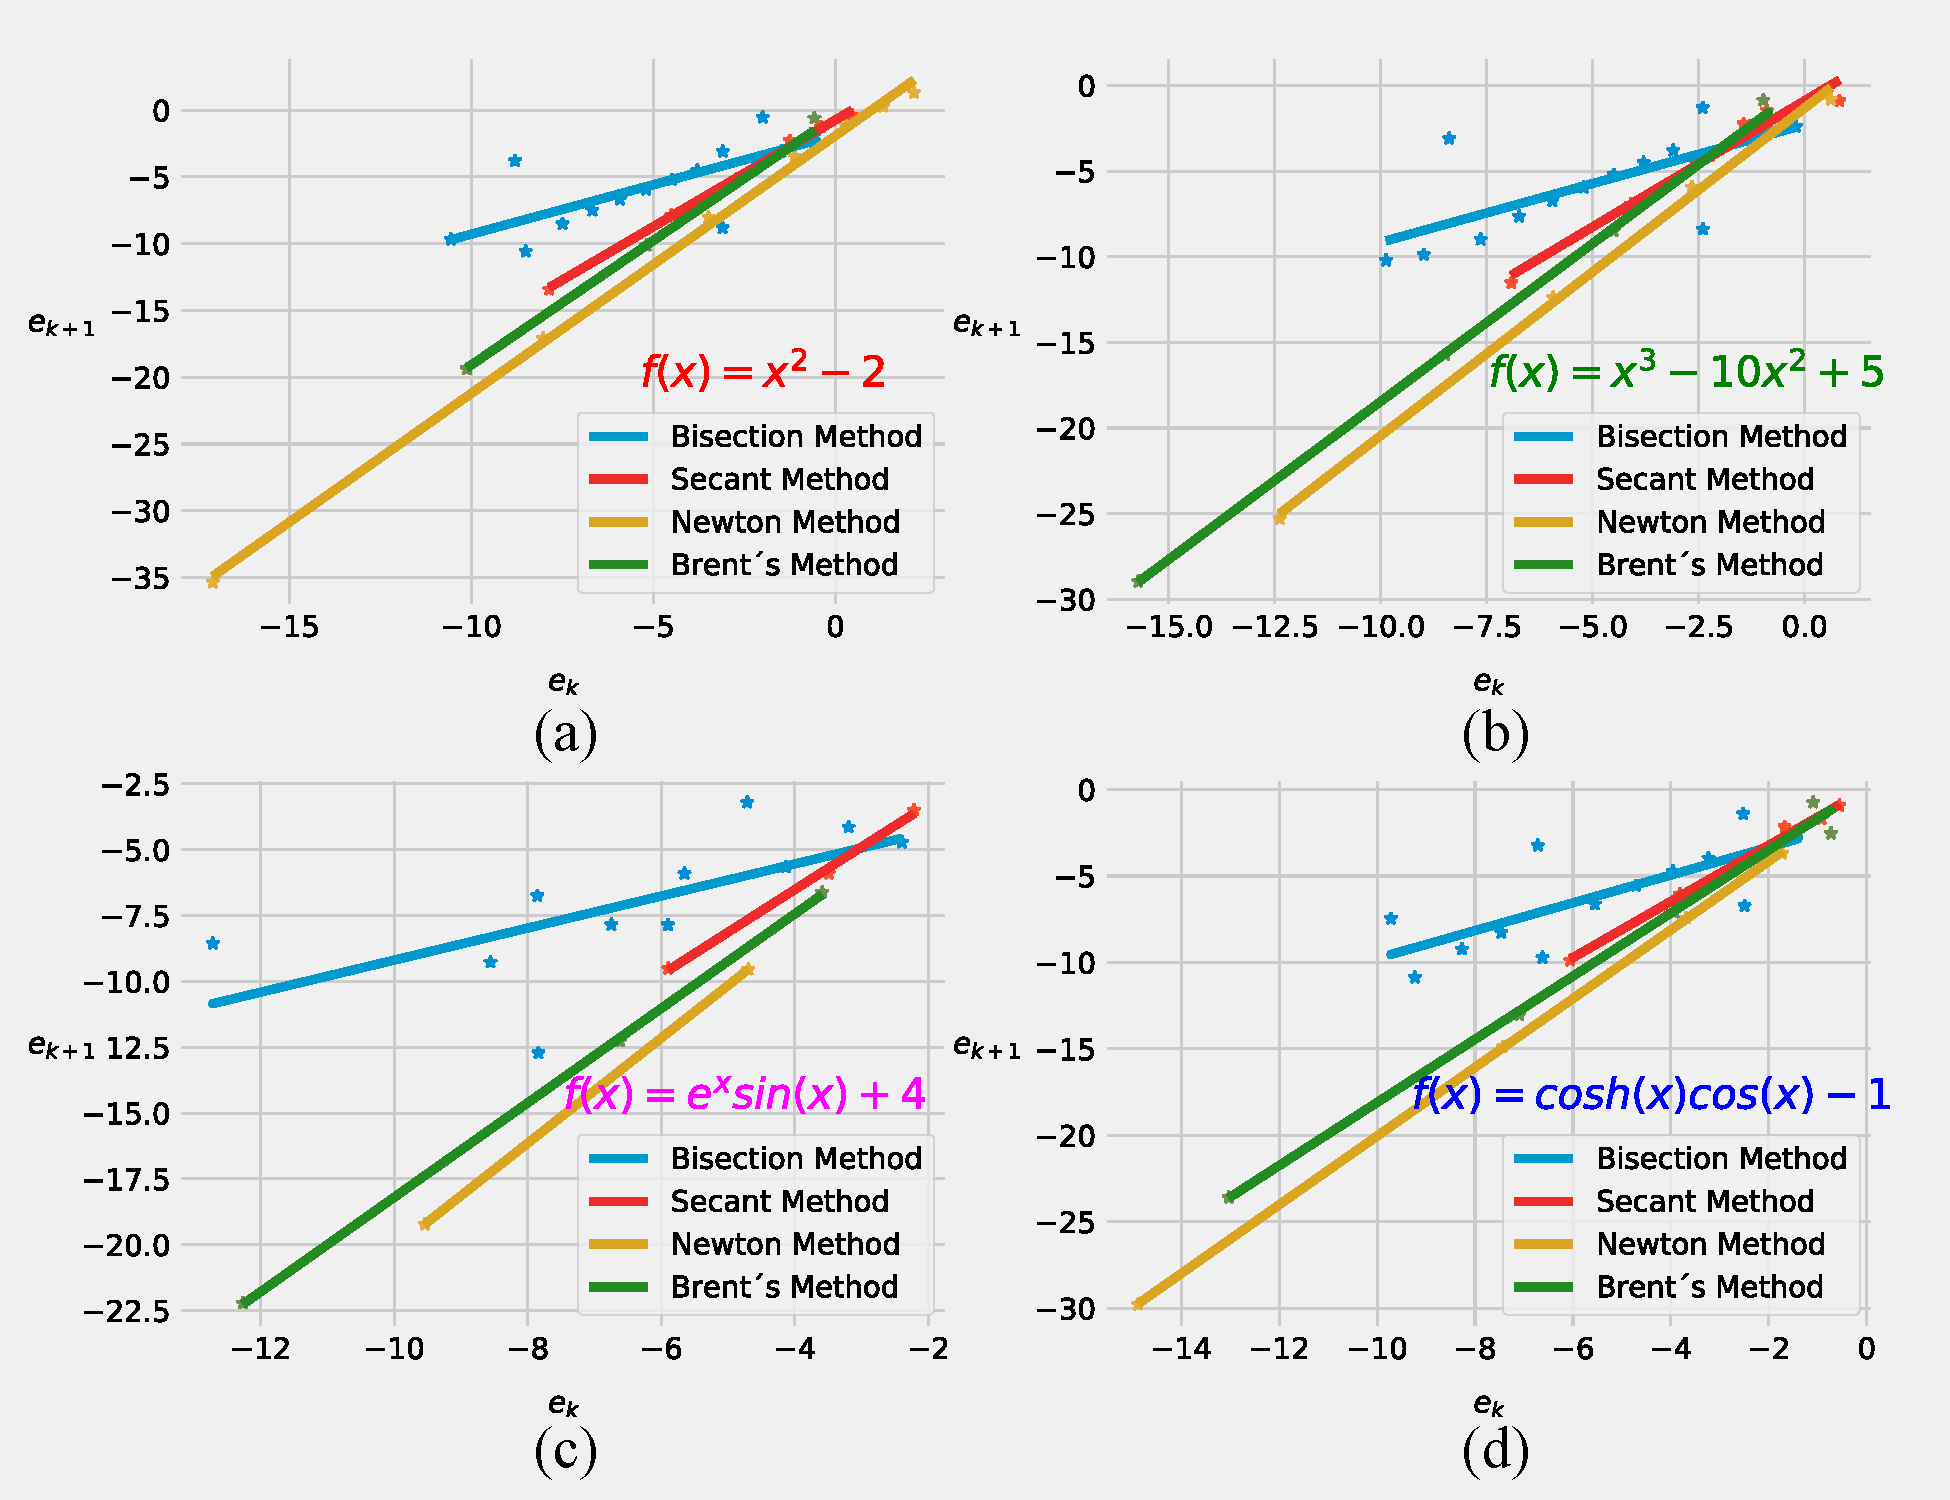
\includegraphics[width=12cm]{img/ErrVsErr1.pdf}\caption{Comparison between the logarithms of $e_{k+1}$ and $e_k$ using different root-finding algorithms and functions. }\label{fig:errVserr}
\end{figure}

\begin{figure}[!h]
	\centering
	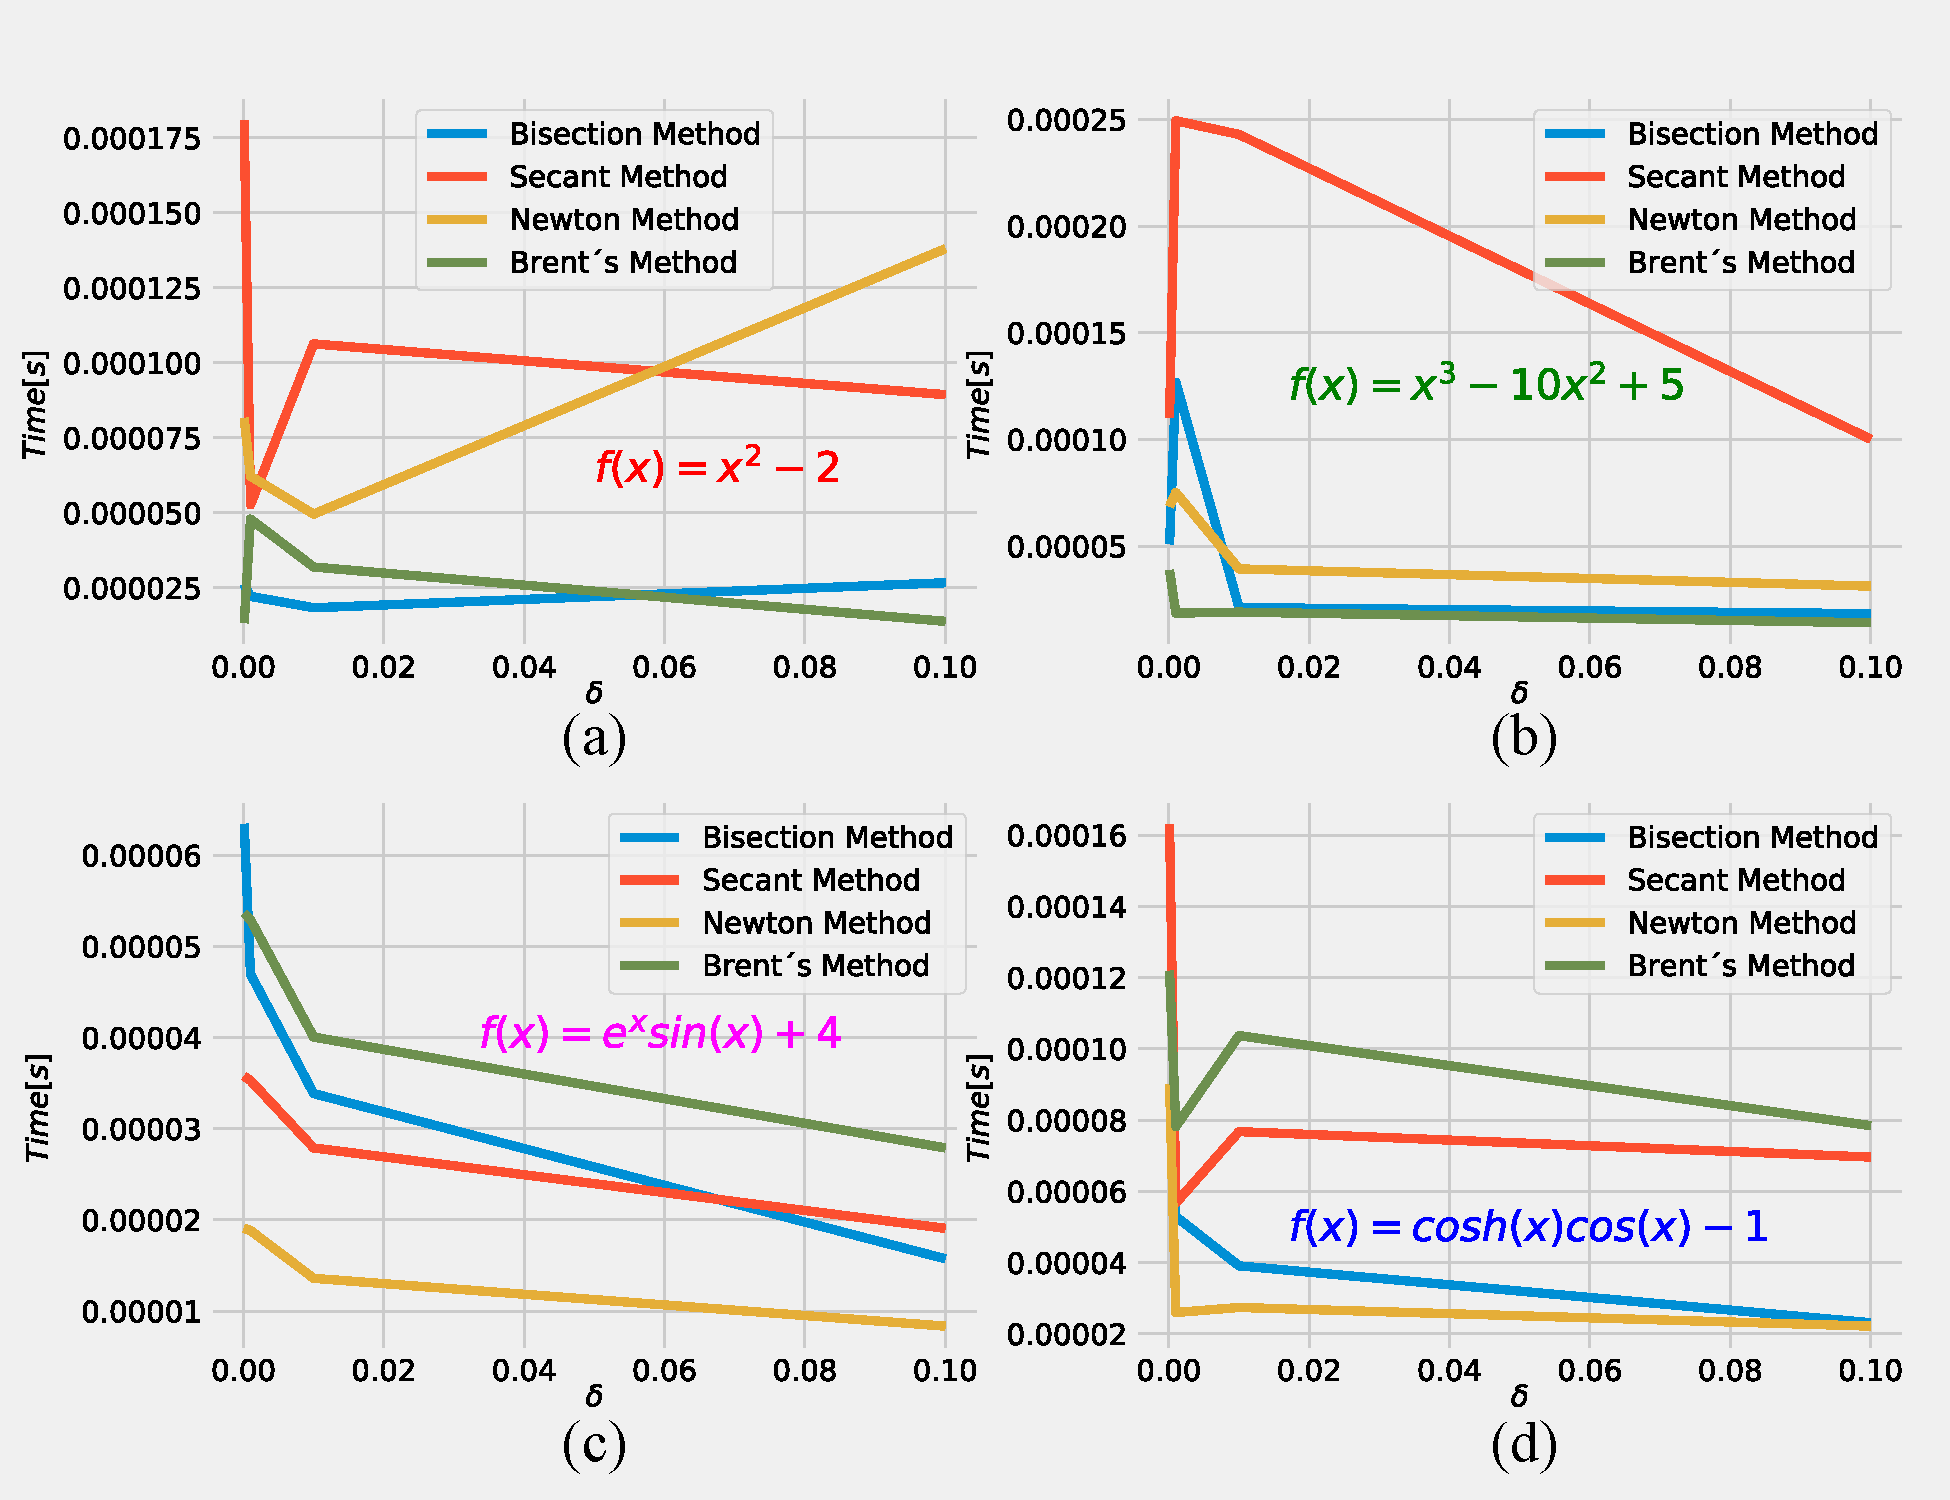
\includegraphics[width=12cm]{img/TimeVsDelta.pdf}\caption{Comparison between perform time and $\delta$ using different root-finding algorithms and functions. }\label{fig:timeVsdelta}
\end{figure}


\end{document}